\subsection{UC11 - Visualizzazione elenco risultati ricerca scaffalatura}
\begin{figure}[H]
  \centering
  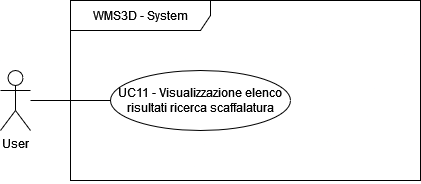
\includegraphics[width=0.8\textwidth]{UC_diagrams_11-20/UC11_sys.drawio.png}
   \caption{Diagramma UML UC11 - Visualizzazione elenco risultati ricerca scaffalatura}
\end{figure}
\begin{figure}[H]
  \centering
  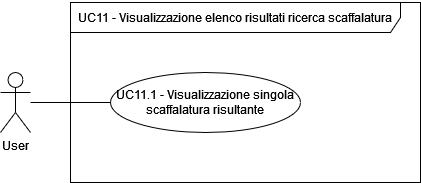
\includegraphics[width=0.8\textwidth]{UC_diagrams_11-20/UC11.drawio.png}
   \caption{Diagramma UML in dettaglio UC11 - Visualizzazione elenco risultati ricerca scaffalatura}
\end{figure}
\begin{itemize}
    \item \textbf{Attori:} User.
    \item \textbf{Pre-condizione:} L'utente ha ricercato una scaffalatura [UC10].
    \item \textbf{Post-condizione:} L'utente visualizza un elenco delle scaffalature il cui codice corrisponde alla ricerca effettuata.
    \item \textbf{Scenario Principale:} L'utente, dopo aver ricercato un determinato codice, visualizza un elenco delle possibili scaffalature corrispondenti alla ricerca, sempre se presenti. Se non ve ne dovesse essere nessuna, l'elenco sarà nullo.
    \item \textbf{Generalizzazioni:} -
    \item \textbf{Estensioni:} -
\end{itemize}


\subsection{UC11.1 - Visualizzazione singola scaffalatura risultante}
\begin{itemize}
    \item \textbf{Attori:} User.
    \item \textbf{Pre-condizione:} L'utente ha ricercato una scaffalatura [UC10] e sta visualizzando l'elenco dei risultati corrispondenti [UC11]. Almeno una scaffalatura deve essere creata [UC6] e posizionata [UC7].
    \item \textbf{Post-condizione:} La scaffalatura risultante dalla ricerca viene selezionata [UC8].
    \item \textbf{Scenario Principale:} Per ogni singola scaffalatura risultante dalla ricerca, l'utente ne visualizza il codice e questa viene selezionata sia in libreria sia nel render 3D.
    \item \textbf{Generalizzazioni:} -
    \item \textbf{Estensioni:} -
\end{itemize}
